%%%%%%%%%%%%%%%%%%%%%%%%%%%%%%%%%%%%%%%%%%%%%%%%%%%%%%%%%%%%%%%%%%%%%%%%%%%%%%%
%%%%%%%%%%%%%%%%%%%%%%%%%%%%%%%%%%%%%%%%%%%%%%%%%%%%%%%%%%%%%%%%%%%%%%%%%%%%%%%
\subsection{Defining the Network and its Parameters}
%%%%%%%%%%%%%%%%%%%%%%%%%%%%%%%%%%%%%%%%%%%%%%%%%%%%%%%%%%%%%%%%%%%%%%%%%%%%%%%
%%%%%%%%%%%%%%%%%%%%%%%%%%%%%%%%%%%%%%%%%%%%%%%%%%%%%%%%%%%%%%%%%%%%%%%%%%%%%%%
As this work constitues the first step towards network analysis using this tracking data I chose to infer a time-aggregated spatial proximity network.
Accordingly, the interactions are undirected but weighted.
A node in the network is a bee, identified by an ID.
The network consists only of bees that interact with other bees at least once, during the specified time interval.

Two bees are associated (spatially close to each other) if their distance is smaller than a \emph{maximum distance}.
Using only this criterion leads to many interactions, resulting in a very dense network, because an interaction could only last for 0.33 seconds.
Therefore, an additional parameter, the \emph{minimum contact duration}, is introduced.
It specifies the minimum time two bees have to spend close to each other to be called associated.

Edges are assigned two attributes.
The first one is the frequency of contacts, meaning how often they share a close position. The second parameter refers to the total duration of contact, so the total time they spend nearby.

%%%%%%%%%%%%%%%%%%%%%%%%%%%%%%%%%%%%%%%%%%%%%%%%%%%%%%%%%%%%%%%%%%%%%%%%%%%%%%%
\subsubsection{Pipeline Parameters}
%%%%%%%%%%%%%%%%%%%%%%%%%%%%%%%%%%%%%%%%%%%%%%%%%%%%%%%%%%%%%%%%%%%%%%%%%%%%%%%
The network pipeline takes two types of parameters. The first set of parameters defines the resulting network and the exact type of spatial proximity. The second set relates to the given data set. Both parameter types are described below.


\begin{table}[htbp]
\small
\centering
\begin{tabularx}{\textwidth}{@{} r Y @{}}
\textbf{Maximum distance} & level of closeness between to individual bees~(in pixel) \vspace{2mm} \\
\textbf{Minimum} & the number of frames two individuals need to spend close\\
\textbf{Contact duration} &  to each other to count it as an interaction ~(in frames) \vspace{2mm} \\
\textbf{Start timestamp} & starting point of the network aggregation~(as UTC string) \vspace{2mm} \\
\textbf{Window size} & size of time window for aggregating the network~(in minutes) \vspace{4mm}\\
\end{tabularx}
\end{table}

\begin{table}[htbp]
\small
\centering
\begin{tabularx}{\textwidth}{@{} r Y @{}}
\textbf{Confidence} & level of confidence, as described in section~\nameref{subsec:confidence}~(in percent) \vspace{2mm}\\
\textbf{Valid IDs} & list of valid ids within a specified time interval, as described in section~\nameref{subsubsec:dataset:filter}~(in CSV file format) \vspace{2mm}\\
\textbf{Gap Size} & for correcting, filling gaps in, the time series of bee pairs~(in frames) \vspace{2mm}\\
\textbf{Number of CPUs} & number of used CPUs for parallelization \vspace{2mm}\\
\textbf{Year} & calculate bee IDs and stitching of camera images according to the observation period~(2015 or 2016)\\
\end{tabularx}
\end{table}

%%%%%%%%%%%%%%%%%%%%%%%%%%%%%%%%%%%%%%%%%%%%%%%%%%%%%%%%%%%%%%%%%%%%%%%%%%%%%%%
\subsubsection{Chosen Parameter Values for Network Analysis}
%%%%%%%%%%%%%%%%%%%%%%%%%%%%%%%%%%%%%%%%%%%%%%%%%%%%%%%%%%%%%%%%%%%%%%%%%%%%%%%
[TODO: muss das nicht zu Method Network Analysis (als ersetr Teil?)]

For network analysis, I chose three days: 20 August, 22 August, and 24. August.
These days were selected because bees from a wide range of age groups were present and older bees, which are likely to be foragers, were more represented in the hive during these days.
Additionally, no data is missing due to camera failures.
The following values are chosen according to biological constraints and similar to other studies, for better comparability.

I chose the length of a bee body, according to \textcite{baracchi2014socio}, as the maximum distance between two bees (Figure~\ref{fig:contactRadius}).
The average bee length of $212$px ($\pm 16$px)  was determined by manually measuring the length of all bees ($n=337$) in images from the four cameras using the tool ImageJ\footnote{\url{http://imagej.net/Welcome}; Last accessed:
 22.02.2016}.
The minimum contact duration is set to three frames (one second). This value corresponds to~\textcite{mersch2013tracking}, as they also exclude interactions below one second.
The networks are aggregated for ten hours during daylight; this corresponds to the biological rhythms of bees.

The confidence level is set to $95\%$, which will keep about 60\% of the data.
The gap size is set to two frames. This value corresponds to the median gap length in the time series of bee pairs.

\begin{figure}[htb]
	\centering
	\begin{subfigure}[b]{0.45\textwidth}
		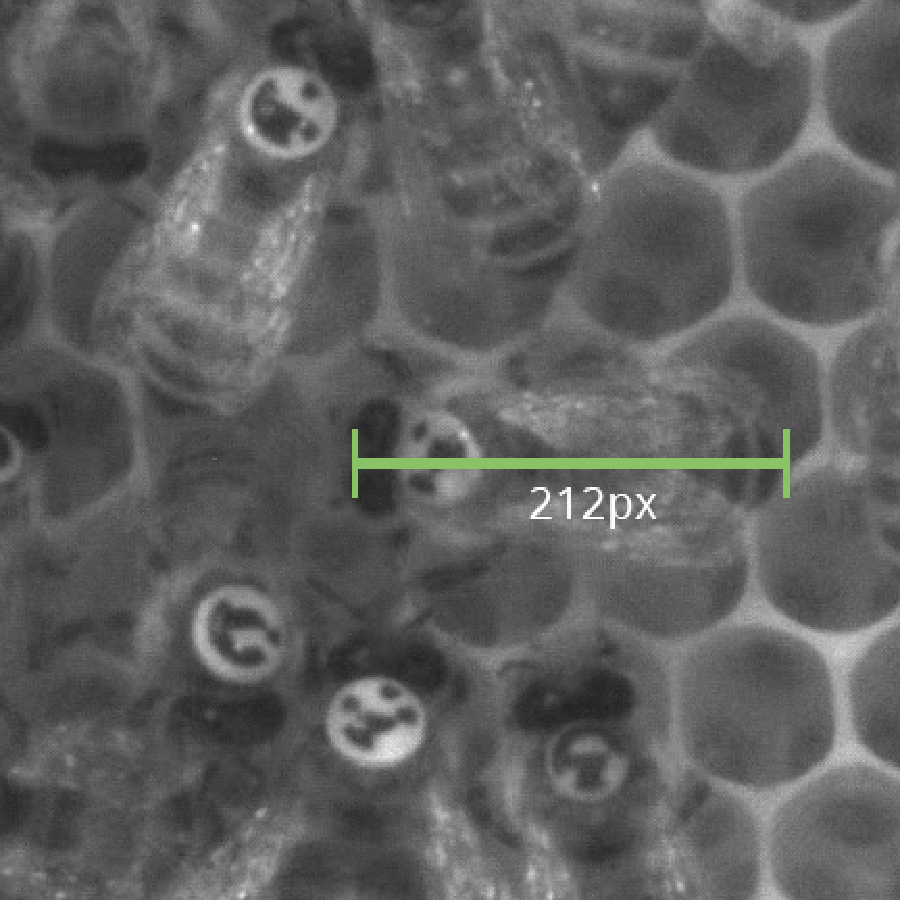
\includegraphics[width=\textwidth]{Figures/sizeTagBee}
		\caption[Body length of a bee]{Body length of a bee}
		\label{fig:size}
	\end{subfigure}
	\hspace{0.08\textwidth}
	\begin{subfigure}[b]{0.45\textwidth}
		\centering
		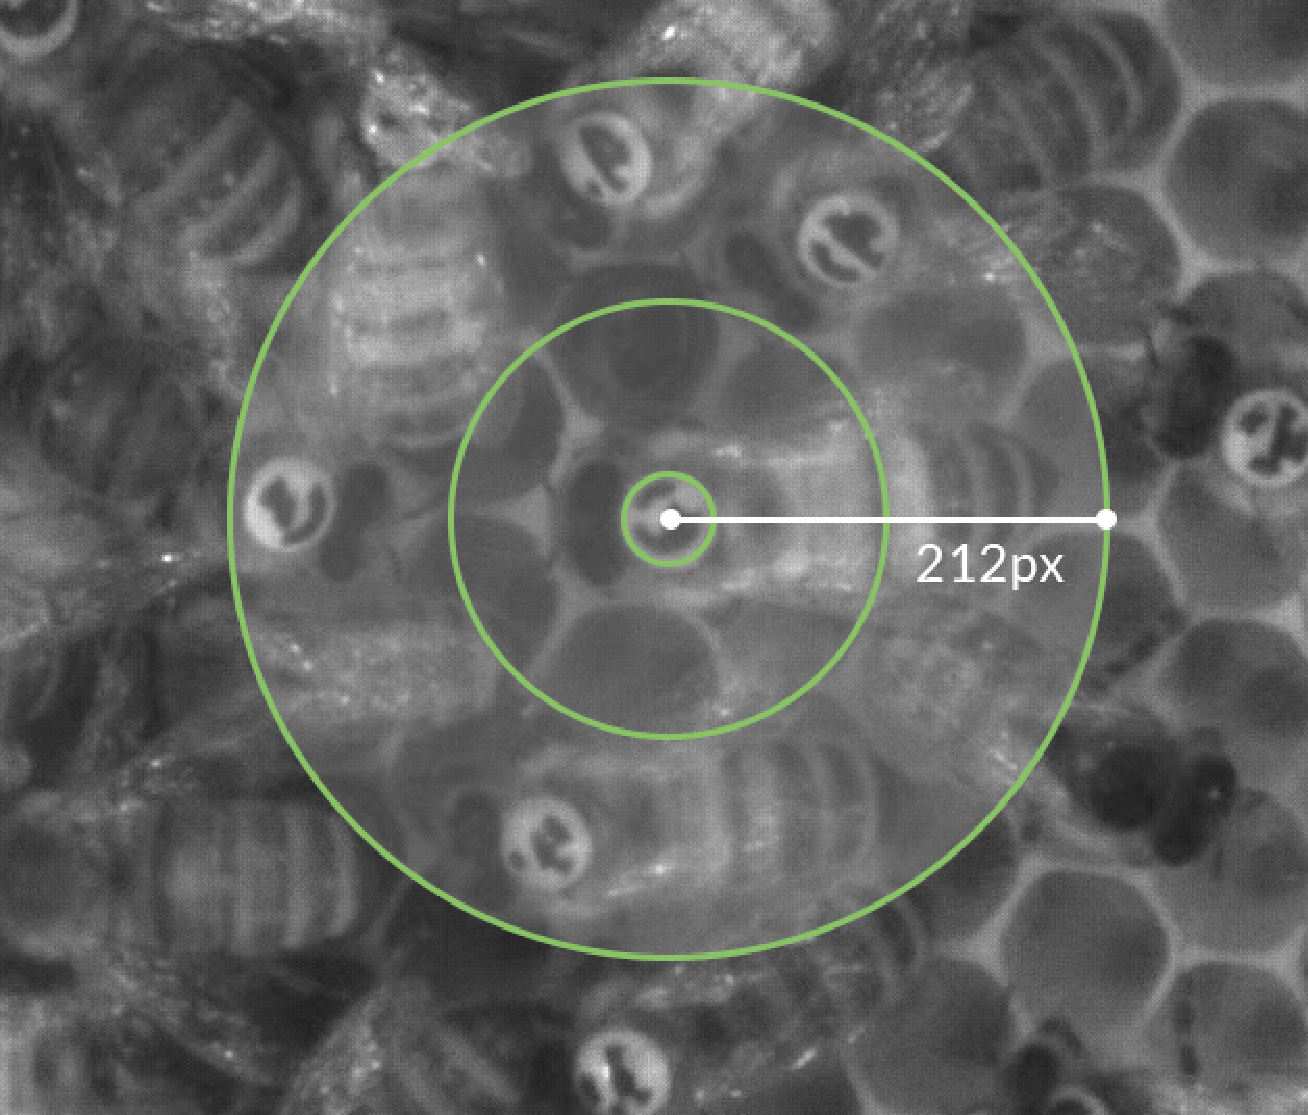
\includegraphics[width=\textwidth]{Figures/radius}
		\caption[Contact radius]{Contact radius}
		\label{fig:radius}
	\end{subfigure}
	\caption[Maximum distance of bees]{\textbf{Maximum distance of bees}: A length of a bee body is chosen as the maximum distance between two bees.}
	\label{fig:contactRadius}
\end{figure}

\begin{table}[htbp]
\small
\centering
\caption[Parameters chosen for network analysis]{\textbf{Parameters chosen for network analysis} The maximum distance corresponds to the length of a bee body and the minimum contact duration is about one second. The networks are aggregated for ten hours.\\
}
\label{tab:chosenparams}

\begin{tabular}{rrl}
	\toprule
	\textbf{Parameter} & \textbf{Value} & \textbf{Unit} \\ \midrule
	Maximum distance & 212 & px \\
	Minimum contact duration & 3 & frames \\
	Window size & 600 & minutes \\ \midrule
	Confidence & 95 & percent \\
	Gap size & 2 & frames \\
	\bottomrule
\end{tabular}

\end{table}